% !TEX TS-program = pdflatex
% !TEX encoding = UTF-8 Unicode

% This is a simple template for a LaTeX document using the "article" class.
% See "book", "report", "letter" for other types of document.

\documentclass[11pt]{article} % use larger type; default would be 10pt

\usepackage[utf8]{inputenc} % set input encoding (not needed with XeLaTeX)

%%% Examples of Article customizations
% These packages are optional, depending whether you want the features they provide.
% See the LaTeX Companion or other references for full information.

%%% PAGE DIMENSIONS
\usepackage{geometry} % to change the page dimensions
\geometry{a4paper} % or letterpaper (US) or a5paper or....
% \geometry{margin=2in} % for example, change the margins to 2 inches all round
% \geometry{landscape} % set up the page for landscape
%   read geometry.pdf for detailed page layout information

\usepackage{graphicx} % support the \includegraphics command and options

% \usepackage[parfill]{parskip} % Activate to begin paragraphs with an empty line rather than an indent

%%% PACKAGES
\usepackage{booktabs} % for much better looking tables
\usepackage{array} % for better arrays (eg matrices) in maths
\usepackage{paralist} % very flexible & customisable lists (eg. enumerate/itemize, etc.)
\usepackage{verbatim} % adds environment for commenting out blocks of text & for better verbatim
\usepackage{subfig} % make it possible to include more than one captioned figure/table in a single float
% These packages are all incorporated in the memoir class to one degree or another...

%%% HEADERS & FOOTERS
\usepackage{fancyhdr} % This should be set AFTER setting up the page geometry
\pagestyle{fancy} % options: empty , plain , fancy
\renewcommand{\headrulewidth}{0pt} % customise the layout...
\lhead{}\chead{}\rhead{}
\lfoot{}\cfoot{\thepage}\rfoot{}

%%% SECTION TITLE APPEARANCE
\usepackage{sectsty}
\allsectionsfont{\sffamily\mdseries\upshape} % (See the fntguide.pdf for font help)
% (This matches ConTeXt defaults)

%%% ToC (table of contents) APPEARANCE
\usepackage[nottoc,notlof,notlot]{tocbibind} % Put the bibliography in the ToC
\usepackage[titles,subfigure]{tocloft} % Alter the style of the Table of Contents
\renewcommand{\cftsecfont}{\rmfamily\mdseries\upshape}
\renewcommand{\cftsecpagefont}{\rmfamily\mdseries\upshape} % No bold!

%%% END Article customizations

\usepackage{epstopdf}

%%% The "real" document content comes below...

\title{Photodiode operation}
\author{Ralph Stevenson-Jones}
%\date{} % Activate to display a given date or no date (if empty),
         % otherwise the current date is printed 

\begin{document}
\maketitle

\section{Introduction}
% \subsection{A subsection}

\section{Calibration against solar cell}

\subsection{Introduction}

In order to obtain the power being supplied by the solar cell from the current generated from the photodiode, the photodiode must be calibrated with the solar cell.  The power management board of the CC5300, used here, sets the operating voltage of the solar cell to a constant voltage, roughly 1.1V, which is at or near the maximum power point of the solar cell for the levels of illumination expected.  The current generated by the solar cell can then be measured using a picco-ammeter and calibrated against the output of the photodiode.

\subsection{Setup}
The photodiode may first be calibrated against the solar cell by directly measuring the photocurrent using a photodiode for a range of light levels.
The photodiode is then subsequently connected to an op-amp within the MSP430 (usually OA0) configured as a trans-impedance amplier with a gain set by the value of the feedback resistor used.
The output of the ti op-amp can then be routed to an ADC within the MSP430 and the digital output displayed through the serial port.

There are thus three different points that the calibration can be made.  It would seem like a good idea to calibrate each in turn as they should all be related by known constants, e.g. the value of the gain in the op-amp, reference voltage and resolution of the ADC.  Each are measured simultaneous to the photocurrent generated by the solar cell when connected to the power management board.

\subsubsection{Direct current measurement}
Here the photodiode is connected directly to an ammeter and the current measured.  As there is no voltage across the ammeter it is in the same configuration as will be used when connected to the ti op-amp.  The layout is shown in Figure \ref{fig:photodiode_solar_cell_calibration_current}
\begin{figure}[htbp]
	\center
	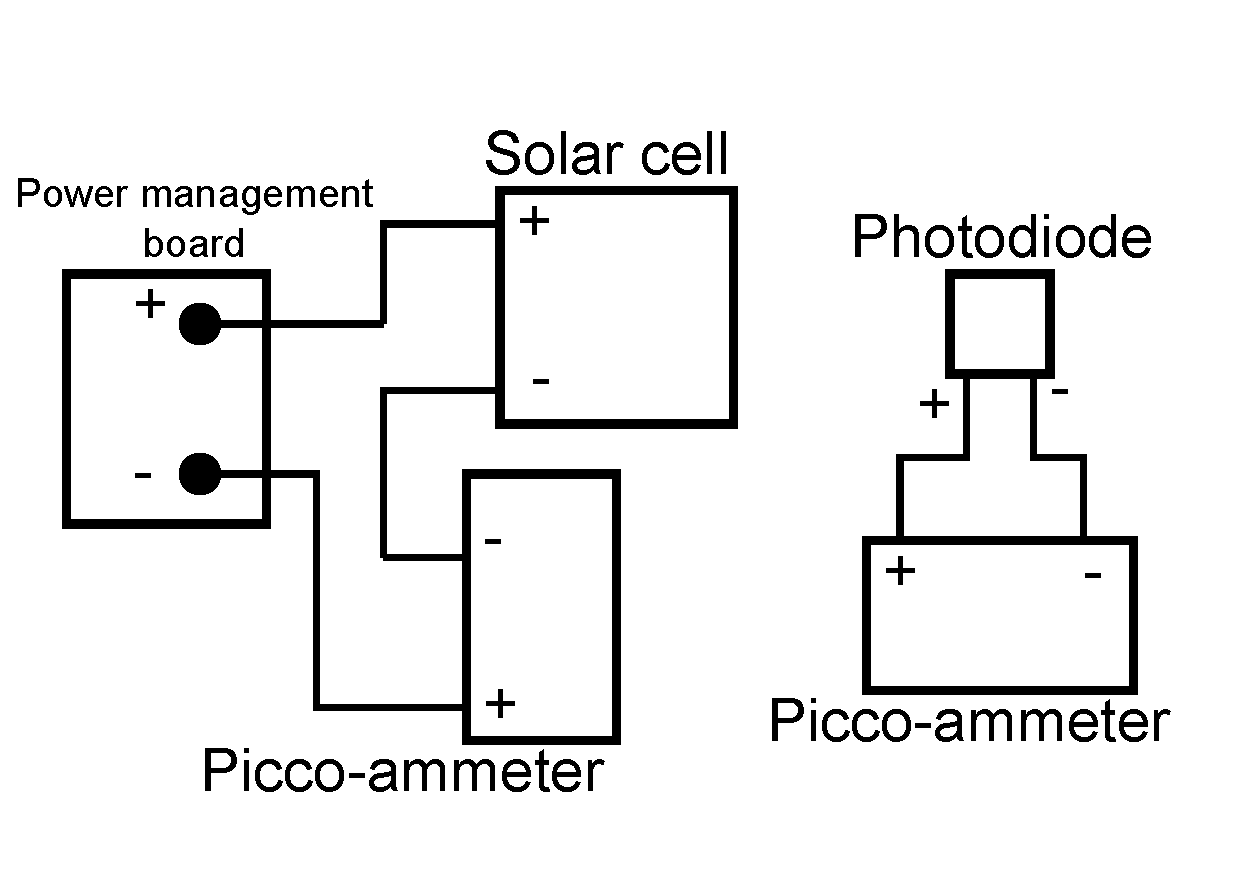
\includegraphics[width = 0.9\textwidth]{../images/photodiode_solar_cell_calibration_current.pdf}
	\caption{Layout of photodiode calibration with solar cell.}
	\label{fig:photodiode_solar_cell_calibration_current}
\end{figure}

\subsubsection{Trans-impedance op-amp voltage measurement}
The setup fo the photodiode with a ti op-amp configured within the MSP430 is shown in Figure \ref{fig:photodiode_solar_cell_calibration_op-amp}.
\begin{figure}[htbp]
	\center
	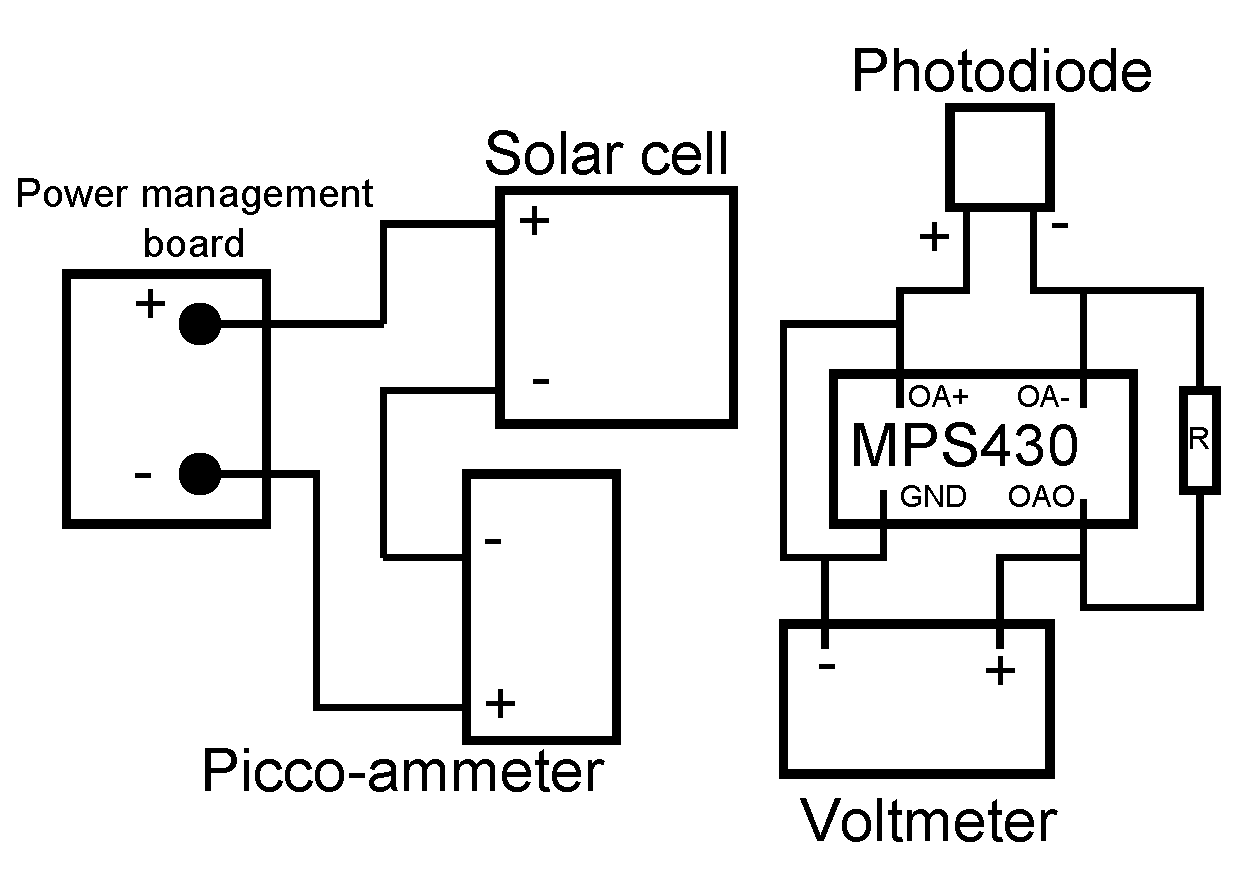
\includegraphics[width = 0.9\textwidth]{../images/photodiode_solar_cell_calibration_op-amp.pdf}
	\caption{Layout of photodiode calibration with solar cell using ti op-amp within MSP430.}
	\label{fig:photodiode_solar_cell_calibration_op-amp}
\end{figure}
The value of the feedback resistor used is 100 k.  The firmware code is saved within \emph{\\CCS\\photodiode\_calibrate}.
\subsubsection{ADC output comparison}
The photodiode is connected to the op-amp and an ADC within the  MSP430 as shown in Figure \ref{fig:photodiode_solar_cell_calibration_adc}.  The digital output from the ADC is then sent through a serial bus and displayed upon the PC.
\begin{figure}[htbp]
	\center
	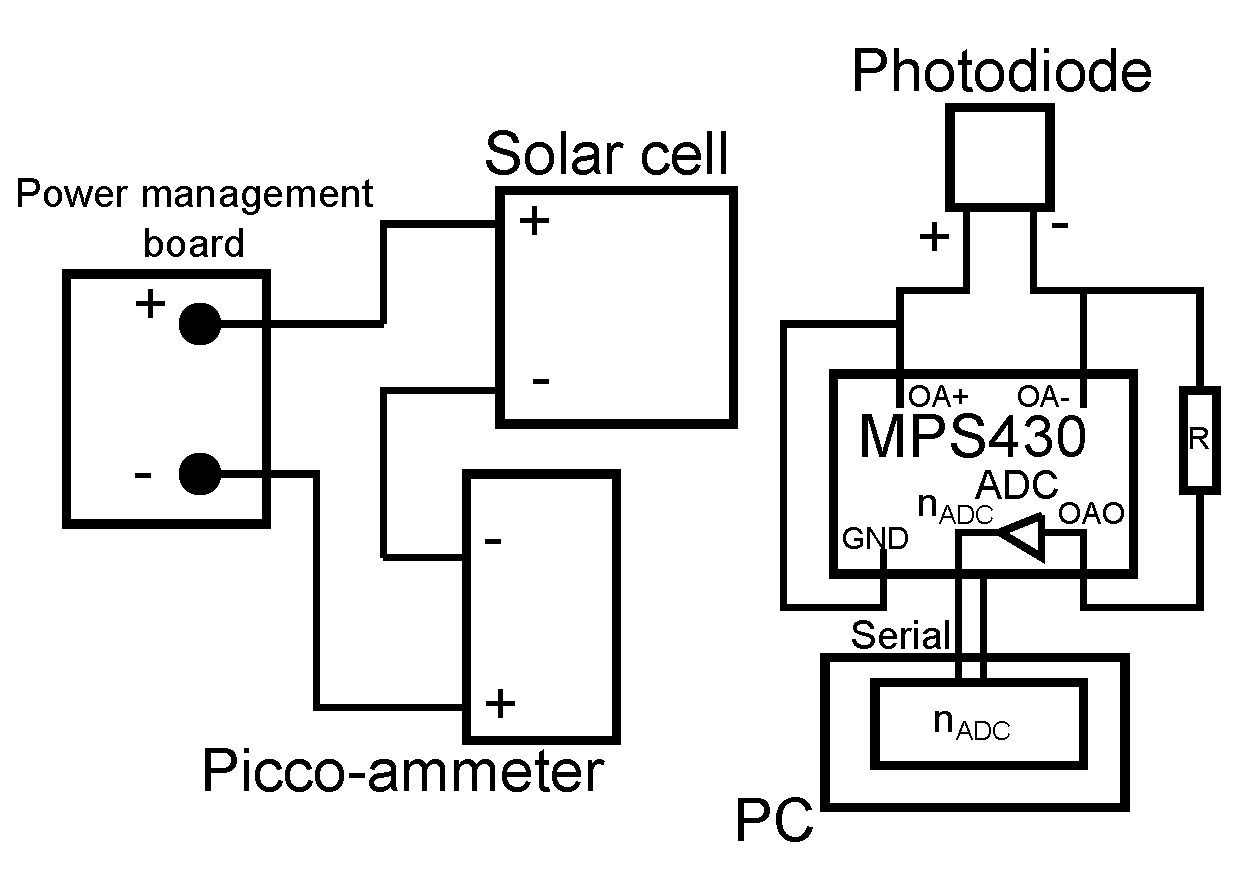
\includegraphics[width = 0.9\textwidth]{../images/photodiode_solar_cell_calibration_adc.pdf}
	\caption{Layout of photodiode calibration with solar cell using ti op-amp and ADC within MSP430.}
	\label{fig:photodiode_solar_cell_calibration_adc}
\end{figure}
The value of the feedback resistor used is 100 k and the reference voltage for the ADC is 1.5V.  The firmware code is saved within the \emph{\$PROJECT-ROOT\$/CCS/photodiode\_test} folder.
\subsection{Results}

\subsubsection{Trans-impedance op-amp voltage measurement}
The solar cell and photodiode were placed next to one-another and illuminated using a halogen lamp.  The lamps was directed at a piece of white paper to create a diffuse light uniform over the area of the solar cell and photodiode.  Data is saved within the file \emph{data\_2015\_10\_27.csv} within the \emph{data} folder.  The data is shown in Figure \ref{fig:data_2015_10_27}.
\begin{figure}[htbp]
	\center
	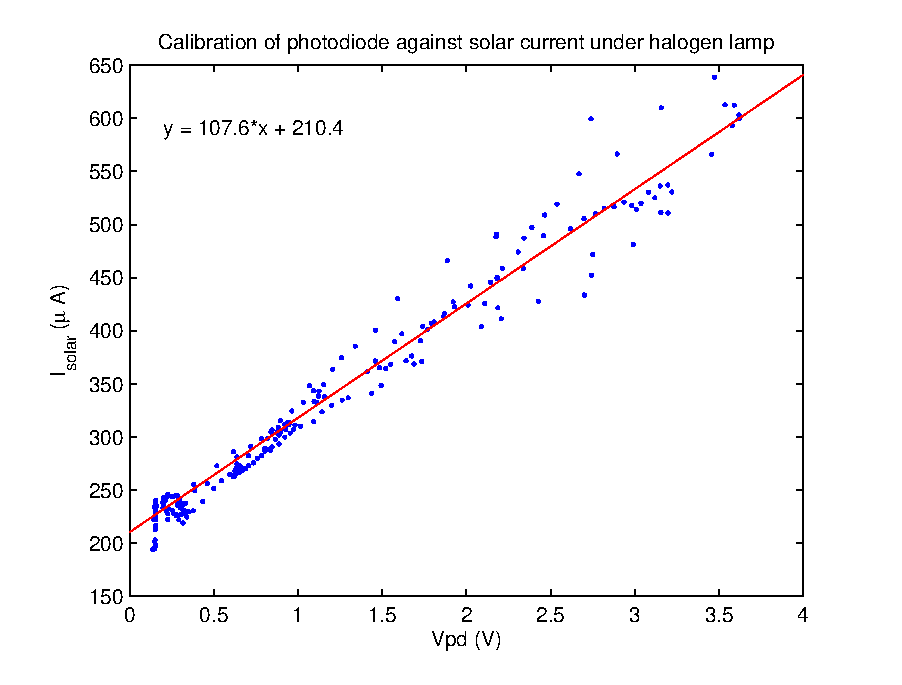
\includegraphics[width = 0.9\textwidth]{../images/data_2015_10_27.eps}
	\caption{Photocurrent as a function of op-amp voltage.}
	\label{fig:data_2015_10_27}
\end{figure}

\subsection{Analysis}
\begin{itemize}
	\item Why is there a y-offset when calibrated against the op-amp voltage (Figure \ref{fig:data_2015_10_27})?
\end{itemize}

\end{document}
